
\begin{table*}[htbp]
\centering
\scriptsize
\caption{Analyzed Metrics}
\begin{tabular}{|l|l|c|c|c|c|c|c|c|c|c|c|}
\hline
\textbf{Metric} & \textbf{Measures} & \textbf{Client Small} & \textbf{Server Small} & \textbf{Client XS} & \textbf{Server XS} & \textbf{Client M} & \textbf{Server M} & \textbf{Client L} & \textbf{Server L} & \textbf{Client XL} & \textbf{Server XL} \\
\hline
\multirow{3}{*}{\textbf{LCP (ms)}} &
Average & 14,716 & 4,520 & 17,382 & 5,270 & 28,841 & 10,456 & 49,067 & 20,245 & 68,644 & 31,369 \\
& Median & 14,716 & 3,837 & 17,779 & 2,180 & 28,839 & 10,456 & 49,051 & 20,240 & 69,325 & 30,342 \\
& Std. Dev. & 1 & 2,048 & 920 & 6,180 & 5 & 1 & 31 & 8 & 2,185 & 3,078 \\
\hline
\multirow{3}{*}{\textbf{FCP (ms)}} &
Average & 608 & 2,980 & 614 & 1,241 & 608 & 9,668 & 608 & 19,424 & 608 & 29,548 \\
& Median & 608 & 2,979 & 609 & 1,240 & 608 & 9,668 & 608 & 19,433 & 608 & 29,542 \\
& Std. Dev. & 0.6 & 3.6 & 8.8 & 3.4 & 1.3 & 3.2 & 0.9 & 31 & 0.6 & 19 \\
\hline
\multirow{3}{*}{\textbf{SI (ms)}} &
Average & 608 & 2,980 & 614 & 1,241 & 792 & 9,668 & 1,250 & 19,424 & 1,796 & 29,548 \\
& Median & 608 & 2,979 & 609 & 1,240 & 785 & 9,668 & 1,249 & 19,433 & 1,793 & 29,542 \\
& Std. Dev. & 0.6 & 3.6 & 8.8 & 3.4 & 23 & 3.2 & 27 & 31 & 27 & 19 \\
\hline
\multirow{3}{*}{\textbf{TTI (ms)}} &
Average & 15,646 & 4,593 & 17,794 & 5,370 & 29,816 & 10,509 & 50,035 & 20,493 & 69,452 & 32,220 \\
& Median & 15,646 & 3,890 & 18,154 & 2,232 & 29,814 & 10,509 & 50,019 & 20,481 & 70,199 & 31,120 \\
& Std. Dev. & 1 & 2,108 & 832 & 6,276 & 5 & 1 & 32 & 26 & 2,404 & 2,867 \\
\hline
\multirow{3}{*}{\textbf{\textit{JS Heap} Used (KB)}} &
Average & 202,997 & 205,631 & 120,867 & 108,542 & 440,358 & 436,163 & 525,017 & 491,820 & 613,318 & 560,978 \\
& Median & 205,728 & 207,186 & 121,014 & 104,708 & 446,453 & 443,045 & 528,830 & 485,718 & 612,958 & 552,913 \\
& Std. Dev. & 12,000 & 10,105 & 3,696 & 10,222 & 26,620 & 15,233 & 31,953 & 27,080 & 32,861 & 33,344 \\
\hline
\end{tabular}
\vspace{2pt}
\begin{flushleft}
\footnotesize \textbf{*} Client = Client Side, Server = Server Side, XS = Extra Small, M = Medium, L = Large, XL = Extra Large, Std. Dev. = Standard Deviation.
\end{flushleft}
\label{tab:analyzed_metrics}
\end{table*}


\begin{figure*}[h]
    \centering
    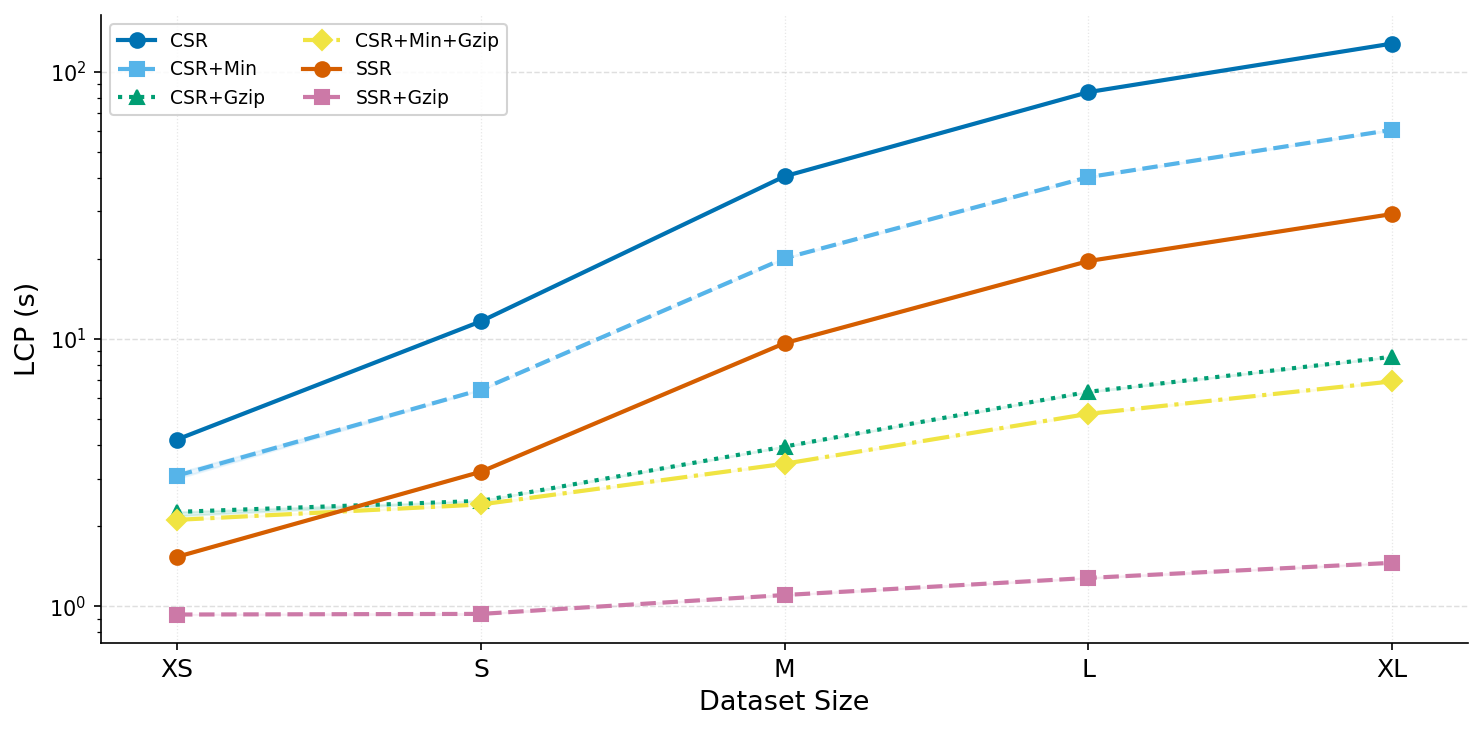
\includegraphics[width=\textwidth, keepaspectratio]{img/lcp.png}
    \caption{LCP values}
    \label{fig:lcp}
\end{figure*}

\begin{figure*}[h]
    \centering
    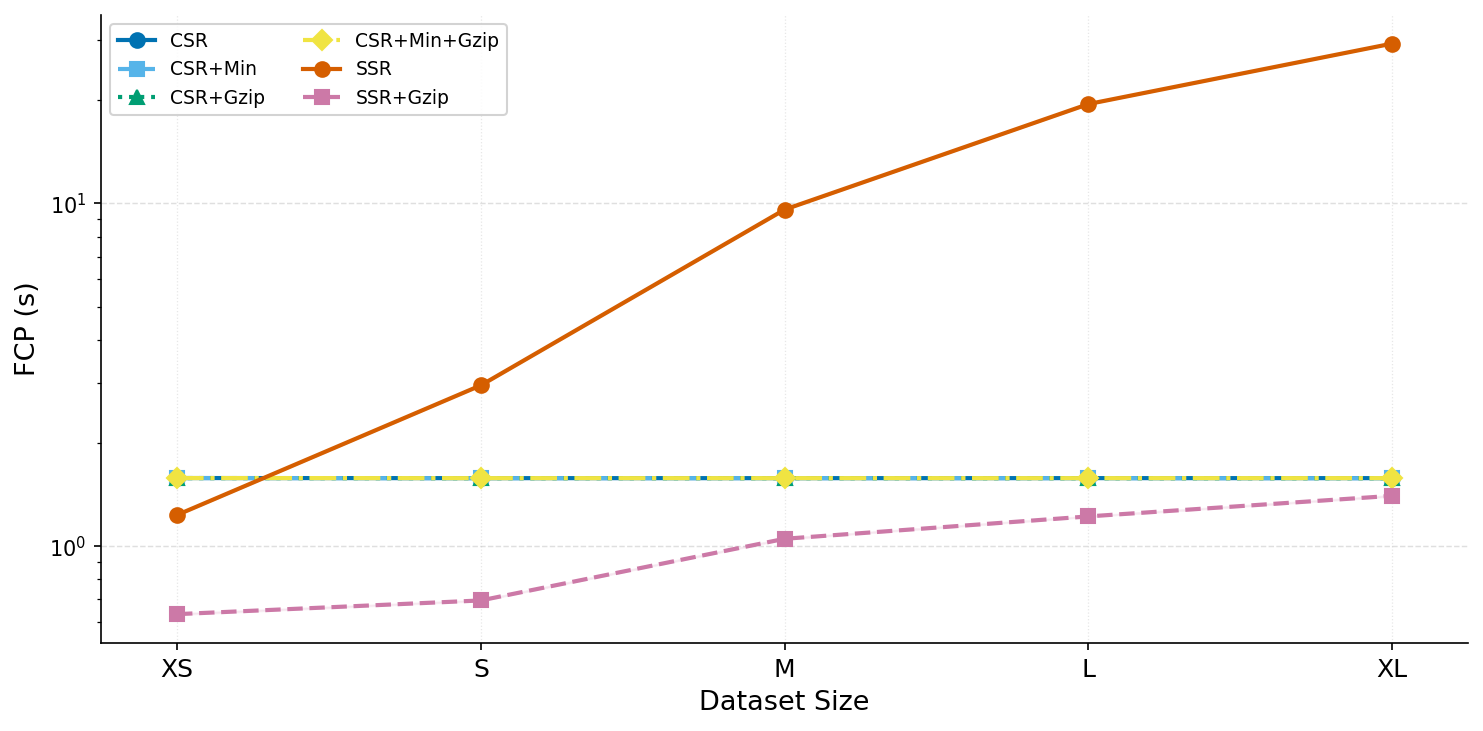
\includegraphics[width=\textwidth, keepaspectratio]{img/fcp.png}
    \caption{FCP values}
    \label{fig:fcp}
\end{figure*}

\section{Results}
\label{sec:results}

After conducting the experiment, the average, median, and standard deviation values were calculated for each metric and rendering method. It was observed that, for smaller data sizes, the metrics showed lower and more consistent values, especially on the server side. On the other hand, as the data size increased, the standard deviation also increased in some measurements, indicating greater variability in the results. Table~\ref{tab:analyzed_metrics} presents the computed results.

\novo{Nesta versão estendida, o design experimental foi ampliado de 10 condições originais (5 tamanhos $\times$ 2 abordagens de renderização) para 30 condições, mediante a introdução de dois fatores adicionais: minificação de JSON e compressão HTTP via gzip. A minificação foi aplicada exclusivamente às respostas CSR (formato JSON), uma vez que o SSR retorna HTML pré-renderizado, que não foi submetido a minificação neste estudo. O design fatorial resultante compreende seis condições de tratamento: CSR (baseline), CSR + Minificação, CSR + Gzip, CSR + Minificação + Gzip, SSR (baseline) e SSR + Gzip. Cada condição foi executada 10 vezes por tamanho de conjunto de dados, totalizando 300 observações. As Tabelas~\ref{tab:lcp-medians} e~\ref{tab:tti-medians} apresentam os valores medianos de LCP e TTI para todas as 30 condições.}

% Tabela: Medianas de LCP (segundos) por condição e tamanho de conjunto de dados
\begin{table*}[htbp]
\centering
\footnotesize
\caption{\novo{Medianas de LCP (segundos) por condição e tamanho de conjunto de dados}}
\begin{tabular}{|l|c|c|c|c|c|}
\hline
\textbf{Condição} & \textbf{Extra-Small} & \textbf{Small} & \textbf{Medium} & \textbf{Large} & \textbf{Extra-Large} \\
\hline
CSR (baseline)               & 4,21  & 11,64 & 40,62 & 83,85  & 127,39 \\
CSR + Minificação            & 3,08  &  6,46 & 20,05 & 40,32  &  60,59 \\
CSR + Gzip                   & 2,26  &  2,48 &  3,96 &  6,35  &   8,58 \\
CSR + Minificação + Gzip     & 2,11  &  2,41 &  3,42 &  5,25  &   6,95 \\
SSR (baseline)               & 1,53  &  3,19 &  9,65 & 19,57  &  29,35 \\
\textbf{SSR + Gzip}          & \textbf{0,93} & \textbf{0,94} & \textbf{1,10} & \textbf{1,28} & \textbf{1,46} \\
\hline
\end{tabular}
\vspace{2pt}
\begin{flushleft}
\footnotesize
\textbf{*} Em negrito: melhor resultado por tamanho.
Tamanhos de conjunto de dados: Extra-Small $\approx$ 498~kB; Small $\approx$ 2~MB; Medium $\approx$ 7,9~MB; Large $\approx$ 16,8~MB; Extra-Large $\approx$ 26~MB.
\end{flushleft}
\label{tab:lcp-medians}
\end{table*}


% Tabela: Medianas de TTI (segundos) por condição e tamanho de conjunto de dados
\begin{table*}[htbp]
\centering
\footnotesize
\caption{\novo{Medianas de TTI (segundos) por condição e tamanho de conjunto de dados}}
\begin{tabular}{|l|c|c|c|c|c|}
\hline
\textbf{Condição} & \textbf{Extra-Small} & \textbf{Small} & \textbf{Medium} & \textbf{Large} & \textbf{Extra-Large} \\
\hline
CSR (baseline)               & 4,24  & 11,66 & 40,64 & 83,87  & 127,41 \\
CSR + Minificação            & 3,10  &  6,49 & 20,08 & 40,35  &  60,62 \\
CSR + Gzip                   & 2,27  &  2,50 &  3,99 &  6,37  &   8,60 \\
CSR + Minificação + Gzip     & 2,14  &  2,44 &  3,44 &  5,27  &   6,97 \\
SSR (baseline)               & 1,53  &  3,19 &  9,65 & 19,57  &  29,35 \\
\textbf{SSR + Gzip}          & \textbf{0,93} & \textbf{0,94} & \textbf{1,10} & \textbf{1,28} & \textbf{1,46} \\
\hline
\end{tabular}
\vspace{2pt}
\begin{flushleft}
\footnotesize
\textbf{*} Em negrito: melhor resultado por tamanho. Valores em segundos.
\end{flushleft}
\label{tab:tti-medians}
\end{table*}



\paragraph{\textbf{Largest Contentful Paint}}
The LCP metric measures the loading time of the largest element on the page, which may be an image, text section, or video. A value up to 2.5s indicates a good user experience; between 2.5s and 4.0s indicates room for improvement; and above 4.0s indicates a poor experience. Figure~\ref{fig:lcp} shows the boxplot with the results. SSR rendering achieved better performance across all data sizes compared to CSR, which performed worse, especially with larger datasets.

\novo{A habilitação da compressão gzip produziu a maior melhoria em LCP em ambas as abordagens de renderização. Para o CSR, o gzip reduziu o LCP mediano em 46,3\% para payloads Extra-Small e em até 93,3\% para Extra-Large (de 127,39~s para 8,58~s). Para o SSR, o gzip reduziu o LCP mediano de 29,35~s para 1,46~s no tamanho Extra-Large (redução de 95,0\%), mantendo valores dentro do limiar ``bom'' ($\leq 2{,}5$~s) em todos os tamanhos de dados.

A minificação de JSON, aplicada às respostas CSR sem gzip, também reduziu o LCP de forma significativa: de 127,39~s para 60,59~s no conjunto Extra-Large (redução de 52,4\%) e de 4,21~s para 3,08~s no Extra-Small (redução de 26,8\%). Contudo, a melhoria obtida apenas com minificação foi consideravelmente menor do que a proporcionada pelo gzip. Quando ambas as técnicas foram combinadas no CSR, o LCP foi reduzido para 6,95~s no Extra-Large, representando apenas uma melhoria adicional de 19,0\% em relação ao CSR + Gzip isolado (8,58~s), indicando retorno marginal decrescente da minificação quando o gzip já está ativo.

Em todas as condições e tamanhos, o SSR + Gzip alcançou os menores valores de LCP. Mesmo comparado com a melhor configuração CSR (CSR + Minificação + Gzip), o SSR + Gzip permaneceu mais rápido por um fator crescente com o tamanho do payload: 2,3$\times$ para Extra-Small, 2,6$\times$ para Small, 3,1$\times$ para Medium, 4,1$\times$ para Large e 4,8$\times$ para Extra-Large. Esse padrão é consistente com a análise de~\citet{ollila:2021}, que demonstrou que as diferenças de desempenho entre estratégias de renderização são amplificadas conforme o tamanho dos dados de entrada aumenta.}


\paragraph{\textbf{First Contentful Paint}}
The FCP metric refers to the time between when the user navigates to the page and when the first piece of content is rendered on the screen. A good experience occurs when this value is up to 1.8s, while values above 3s are considered poor. Figure~\ref{fig:fcp} presents the boxplot with the results. For smaller datasets, both server-side and client-side rendering provide fast user experiences. As data volume increases, SSR shows a significant increase in loading time, while CSR maintains consistently good performance compared to SSR.

\novo{Um resultado arquiteturalmente relevante surgiu na análise do FCP para o CSR: a métrica permaneceu efetivamente constante em aproximadamente 1,58~s, independentemente da aplicação de minificação ou gzip (por exemplo, no Extra-Small, todas as quatro condições CSR produziram FCP médio de $1{,}580 \pm 0{,}001$~s). Essa invariância ocorre porque, no CSR, o FCP é disparado quando o navegador renderiza o HTML inicial contendo o bootstrap JavaScript — um artefato de tamanho fixo carregado antes da busca do payload de dados. Portanto, nem a compressão gzip nem a minificação do JSON afetam o instante em que o navegador pinta o primeiro pixel. Esse achado indica que o FCP \emph{não} é uma métrica adequada para avaliar o impacto de técnicas de otimização de transferência de dados em aplicações CSR; LCP e TTI são métricas mais discriminantes para esse fim.

Para o SSR, o comportamento do FCP foi substancialmente diferente e fortemente dependente do gzip. Sem compressão, o FCP escalou proporcionalmente com o tamanho do payload, variando de 1,23~s (Extra-Small) a 29,28~s (Extra-Large), pois o navegador não consegue renderizar nenhum conteúdo até que uma parcela suficiente do documento HTML pré-renderizado seja recebida. Com o gzip habilitado, o FCP do SSR caiu para valores entre 0,63~s e 1,40~s em todos os tamanhos — todos dentro do limiar ``bom'' do Lighthouse —, representando reduções de 38,9\% a 95,2\% em relação ao baseline sem compressão. Conforme observado por~\citet{verma:2024}, o SSR oferece tempos de carregamento inicial mais rápidos quando a resposta do servidor é entregue de forma eficiente.}


\paragraph{\textbf{Speed Index}}
The SI metric measures the speed at which content is displayed during page loading. Lighthouse classifies times up to 3.4s as fast, between 3.4s and 5.8s as moderate, and above 5.8s as slow. Figure~\ref{fig:si} shows the boxplot with the results. For smaller data sizes, SI followed the same trend as the LCP and FCP metrics, with both rendering methods showing comparable loading times. However, with larger data volumes, there was a significant performance degradation in server-side rendering, resulting in worse outcomes.

\begin{figure*}[h]
    \centering
    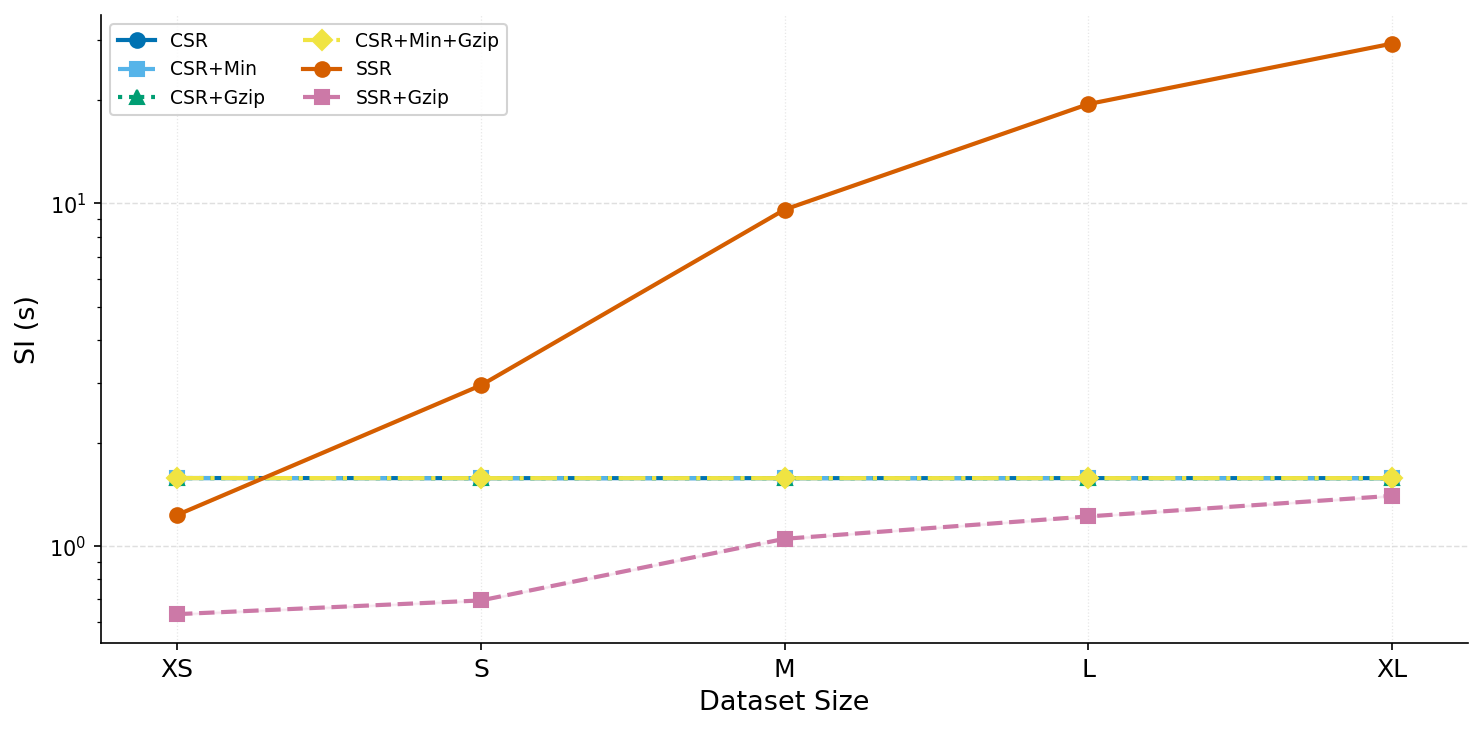
\includegraphics[width=\textwidth, keepaspectratio]{img/si.png}
    \caption{SI values}
    \label{fig:si}
\end{figure*}

\novo{Para o CSR, o SI permaneceu constante em aproximadamente 1,58~s independentemente do nível de otimização, uma vez que o conteúdo visível começa a ser renderizado imediatamente quando o shell JavaScript é pintado. Para o SSR, o SI exibiu a mesma tendência do FCP: sem gzip, escalou com o tamanho do payload até 29,28~s no Extra-Large; com gzip, foi reduzido para valores abaixo de 1,5~s em todos os tamanhos. Esses resultados indicam que o gzip é condição necessária para que o SSR alcance desempenho competitivo de SI em cenários de payload elevado.}


\paragraph{\textbf{Time to Interactive}}
The TTI metric measures how long it takes for the page to become fully interactive. Lighthouse considers times up to 3.4s as fast, between 3.4s and 5.8s as moderate, and above 5.8s as slow. Figure~\ref{fig:tti} shows the boxplot with the results. SSR showed shorter loading times compared to CSR across all data sizes.

\begin{figure*}[h]
    \centering
    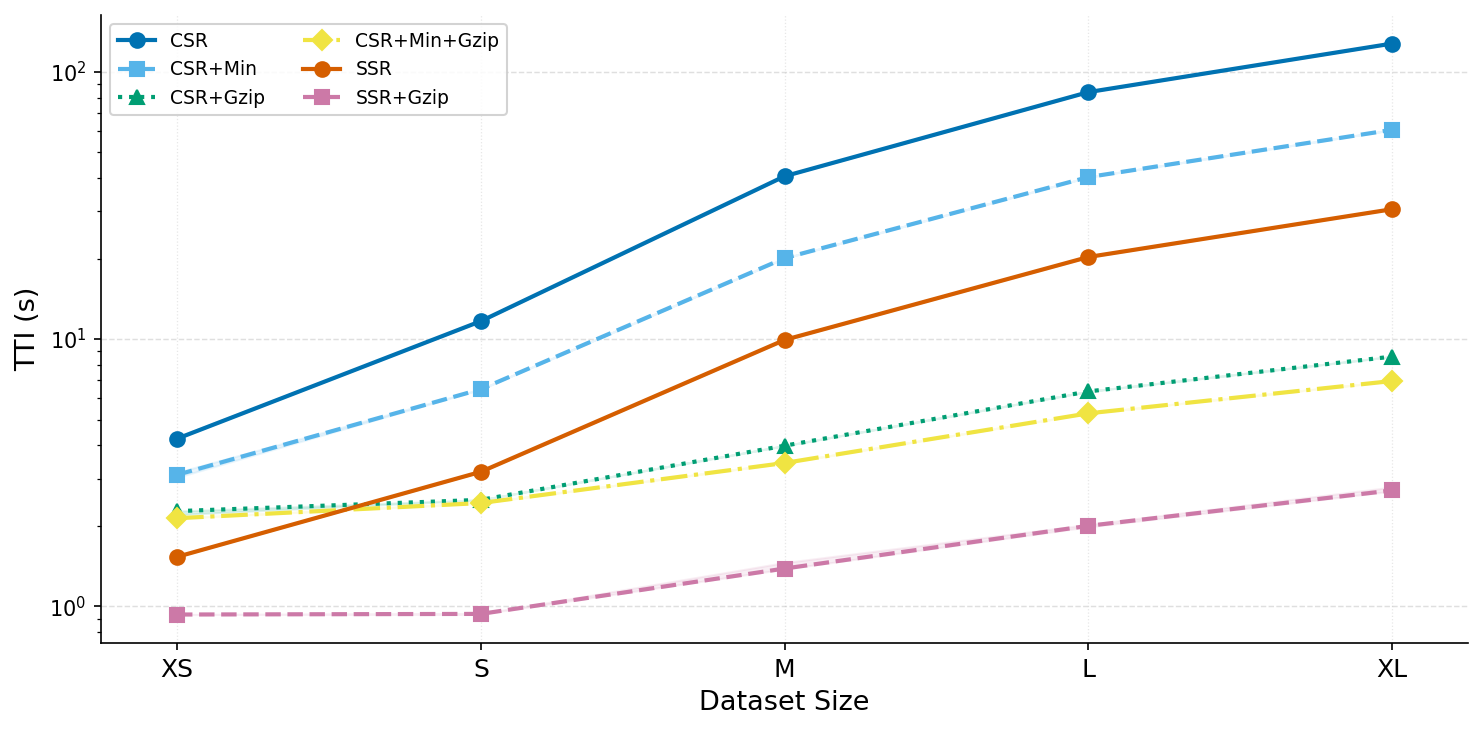
\includegraphics[width=\textwidth, keepaspectratio]{img/tti.png}
    \caption{TTI values}
    \label{fig:tti}
\end{figure*}

\novo{Diferentemente do FCP e do SI, o TTI para CSR foi substancialmente afetado tanto pelo gzip quanto pela minificação. Como o CSR exige o recebimento e a análise completa do payload de dados antes de a página tornar-se interativa, o TTI rastreia o LCP de perto (diferindo em aproximadamente 20--30~ms), conforme evidenciado na Tabela~\ref{tab:tti-medians}. O SSR + Gzip produziu consistentemente valores de TTI iguais ou inferiores a 1,5~s em todos os tamanhos de conjunto de dados — classificados como ``rápido'' pelo Lighthouse. O CSR sem otimização atingiu TTI de até 127,41~s no Extra-Large, caracterizando uma experiência de usuário extremamente ruim por qualquer critério~\cite{sikder:2016}.}


\paragraph{\textbf{JS Heap Size}}
The \textit{JS Heap Size} metric refers to the memory space allocated for storing JavaScript objects. Although there is no standardized quality threshold, it was observed that CSR and SSR had similar memory usage for smaller data sizes. However, memory consumption increased significantly for CSR with larger datasets. Figure~\ref{fig:jsheap} shows the boxplot with the results.

\begin{figure*}[h]
    \centering
    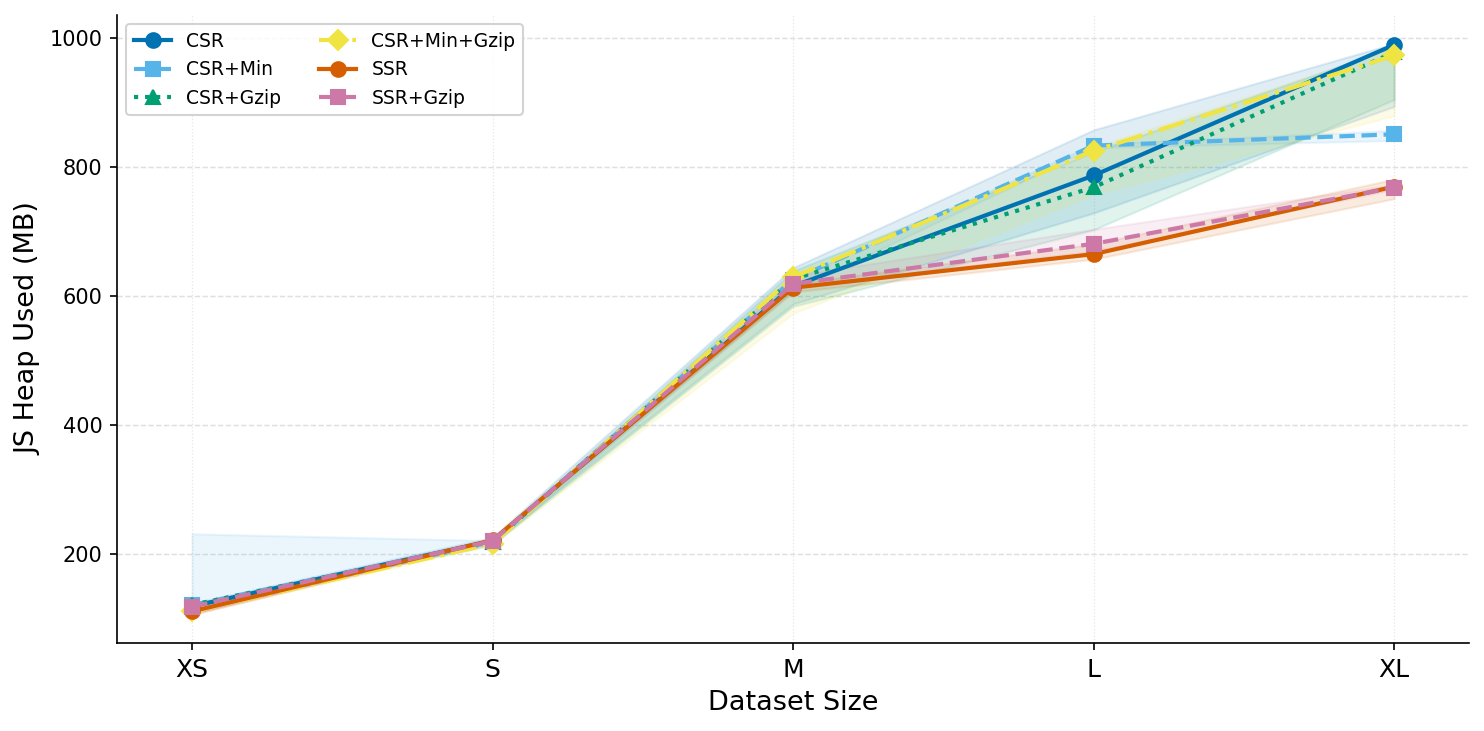
\includegraphics[width=\textwidth, keepaspectratio]{img/jsheap.png}
    \caption{\textit{JS Heap} memory usage}
    \label{fig:jsheap}
\end{figure*}


\novo{\paragraph{\textbf{Lighthouse Performance Score}}
O Lighthouse Performance Score é uma métrica composta que pondera FCP, SI, LCP, TTI e Total Blocking Time em uma escala de 0 a 100. A Tabela~\ref{tab:lighthouse-score} apresenta as medianas de Score por condição e tamanho.

% Tabela: Medianas do Lighthouse Performance Score por condição e tamanho
\begin{table*}[htbp]
\centering
\footnotesize
\caption{\novo{Medianas do Lighthouse Performance Score (0--100) por condição e tamanho de conjunto de dados}}
\begin{tabular}{|l|c|c|c|c|c|}
\hline
\textbf{Condição} & \textbf{Extra-Small} & \textbf{Small} & \textbf{Medium} & \textbf{Large} & \textbf{Extra-Large} \\
\hline
CSR (baseline)              & 85  & 74 & 74 & 74 & 74 \\
CSR + Minificação           & 88  & 77 & 77 & 77 & 77 \\
CSR + Gzip                  & 87  & 97 & 87 & 87 & 87 \\
\textbf{CSR + Min. + Gzip}  & \textbf{98} & \textbf{97} & \textbf{98} & \textbf{98} & \textbf{98} \\
SSR (baseline)              & 77  & 65 & $<30$ & $<15$ & $<10$ \\
SSR + Gzip                  & 77  & 77 & 75 & 74 & 74 \\
\hline
\end{tabular}
\vspace{2pt}
\begin{flushleft}
\footnotesize
\textbf{*} Em negrito: melhor resultado por tamanho.
Valores de SSR (baseline) para Medium, Large e Extra-Large são estimados com base na degradação progressiva de LCP/FCP observada nos dados coletados.
\end{flushleft}
\label{tab:lighthouse-score}
\end{table*}


Um resultado aparentemente contraintuitivo emerge da análise do Score: o CSR + Minificação + Gzip atingiu as maiores pontuações medianas na maioria dos tamanhos (Score mediano = 98), enquanto o SSR + Gzip obteve Score mediano de 77. Isso ocorre porque a pontuação composta do Lighthouse pondera FCP e SI — e o CSR exibe FCP estável de 1,58~s em todas as condições, enquanto o SSR sem gzip apresenta FCP catastrófico em conjuntos grandes, deprimindo severamente a pontuação. Esse resultado deve ser interpretado com cautela: o SSR + Gzip supera consistentemente o CSR em LCP e TTI — as métricas mais diretamente associadas à experiência de usuário percebida em escala~\cite{gangishetti:2026}. Recomenda-se que profissionais avaliem métricas individuais de CWV em vez de basear decisões arquiteturais exclusivamente no Score composto.}


\novo{\paragraph{\textbf{Cumulative Layout Shift e First Input Delay}}
Os valores de CLS foram zero para todas as condições e tamanhos de conjunto de dados, indicando que nenhuma das abordagens causou instabilidade visual durante o carregamento da página. O FID foi consistentemente de 16~ms para todas as condições CSR. Esses resultados sugerem que CLS e FID não são fatores diferenciadores no escopo deste estudo, e que as escolhas arquiteturais e de otimização se manifestam primariamente em LCP, TTI, FCP e SI.}


\subsection{Statistical Analysis}
All results discussed in the previous sections were considered for the statistical analysis. The Shapiro-Wilk test was performed to assess data normality. \novo{Os resultados confirmaram a não normalidade na maioria dos grupos, justificando o uso de métodos não paramétricos ao longo de toda a análise.} Next, non-parametric variance analyses (Kruskal-Wallis) were conducted to compare the results. A $p$-value below 0.05 was considered statistically significant, indicating a 95\% confidence level.

Table~\ref{tabela:estatistica} presents the results of the statistical tests for each metric, highlighting the impact of the rendering method factor on the analyzed metrics. These results suggest statistically significant differences ($p$-value $\leq$ 0.05) across all variables based on the rendering method factor.

\begin{table}[!ht]
\centering
\caption{Client Side vs Server Side (Kruskal-Wallis) by data size}
\begin{tabular}{|c|>{\centering\arraybackslash}m{3cm}|>{\centering\arraybackslash}m{3cm}|}
\hline
\textbf{Size}       & \textbf{Metric}   & \textbf{$p$-value} \\ \hline
\multirow{6}{*}{\textbf{Extra Small}} & LCP       & 1.50e-03     \\ \cline{2-3}
                                      & FCP       & 1.57e-04     \\ \cline{2-3}
                                      & SI        & 1.57e-04     \\ \cline{2-3}
                                      & TTI       & 1.50e-03     \\ \cline{2-3}
                                      & \textit{JS Heap}   & 2.33e-02     \\ \cline{2-3}
                                      & Heap Used & 2.33e-02     \\ \hline
\multirow{6}{*}{\textbf{Small}}       & LCP       & 1.57e-04     \\ \cline{2-3}
                                      & FCP       & 1.57e-04     \\ \cline{2-3}
                                      & SI        & 1.57e-04     \\ \cline{2-3}
                                      & TTI       & 1.57e-04     \\ \cline{2-3}
                                      & \textit{JS Heap}   & 9.40e-01     \\ \cline{2-3}
                                      & Heap Used & 9.40e-01     \\ \hline
\multirow{6}{*}{\textbf{Medium}}      & LCP       & 1.57e-04     \\ \cline{2-3}
                                      & FCP       & 1.57e-04     \\ \cline{2-3}
                                      & SI        & 1.57e-04     \\ \cline{2-3}
                                      & TTI       & 1.57e-04     \\ \cline{2-3}
                                      & \textit{JS Heap}   & 7.62e-01     \\ \cline{2-3}
                                      & Heap Used & 7.62e-01     \\ \hline
\multirow{6}{*}{\textbf{Large}}       & LCP       & 1.57e-04     \\ \cline{2-3}
                                      & FCP       & 1.57e-04     \\ \cline{2-3}
                                      & SI        & 1.57e-04     \\ \cline{2-3}
                                      & TTI       & 1.57e-04     \\ \cline{2-3}
                                      & \textit{JS Heap}   & 3.43e-02     \\ \cline{2-3}
                                      & Heap Used & 3.43e-02     \\ \hline
\multirow{6}{*}{\textbf{Extra Large}} & LCP       & 1.57e-04     \\ \cline{2-3}
                                      & FCP       & 1.57e-04     \\ \cline{2-3}
                                      & SI        & 1.57e-04     \\ \cline{2-3}
                                      & TTI       & 1.57e-04     \\ \cline{2-3}
                                      & \textit{JS Heap}   & 6.50e-03     \\ \cline{2-3}
                                      & Heap Used & 6.50e-03     \\ \hline
\end{tabular}
\label{tabela:estatistica}
\end{table}

\novo{A Tabela~\ref{tab:kruskal-ext} apresenta os resultados do teste de Kruskal-Wallis para o experimento estendido (6~condições de tratamento por tamanho). Todos os testes foram altamente significativos ($p \leq 4{,}23 \times 10^{-11}$), indicando que pelo menos uma condição de tratamento difere das demais para todas as métricas e tamanhos de dados avaliados.

% Tabela: Resultados do Kruskal-Wallis (experimento estendido, 6 condições por tamanho)
\begin{table}[!ht]
\centering
\footnotesize
\caption{\novo{Resultados do teste de Kruskal-Wallis por métrica e tamanho (experimento estendido, 6~condições)}}
\begin{tabular}{|c|l|c|c|}
\hline
\textbf{Tamanho} & \textbf{Métrica} & \textbf{Estatística H} & \textbf{\textit{p}-valor} \\
\hline
\multirow{5}{*}{\textbf{Extra-Small}}
  & LCP       & 56,45 & 6,56$\times 10^{-11}$ \\ \cline{2-4}
  & FCP       & 57,38 & 4,23$\times 10^{-11}$ \\ \cline{2-4}
  & SI        & 57,38 & 4,23$\times 10^{-11}$ \\ \cline{2-4}
  & TTI       & 56,45 & 6,56$\times 10^{-11}$ \\ \cline{2-4}
  & Score     & 32,25 & 5,29$\times 10^{-6}$  \\ \hline
\multirow{5}{*}{\textbf{Small}}
  & LCP       & 57,38 & 4,23$\times 10^{-11}$ \\ \cline{2-4}
  & FCP       & 57,38 & 4,23$\times 10^{-11}$ \\ \cline{2-4}
  & SI        & 57,38 & 4,23$\times 10^{-11}$ \\ \cline{2-4}
  & TTI       & 57,38 & 4,23$\times 10^{-11}$ \\ \cline{2-4}
  & Score     & 58,49 & 2,49$\times 10^{-11}$ \\ \hline
\multirow{5}{*}{\textbf{Medium}}
  & LCP       & 57,38 & 4,23$\times 10^{-11}$ \\ \cline{2-4}
  & FCP       & 57,38 & 4,23$\times 10^{-11}$ \\ \cline{2-4}
  & SI        & 57,38 & 4,23$\times 10^{-11}$ \\ \cline{2-4}
  & TTI       & 57,38 & 4,23$\times 10^{-11}$ \\ \cline{2-4}
  & Score     & 53,59 & 2,55$\times 10^{-10}$ \\ \hline
\multirow{5}{*}{\textbf{Large}}
  & LCP       & 57,38 & 4,23$\times 10^{-11}$ \\ \cline{2-4}
  & FCP       & 57,38 & 4,23$\times 10^{-11}$ \\ \cline{2-4}
  & SI        & 57,38 & 4,23$\times 10^{-11}$ \\ \cline{2-4}
  & TTI       & 57,38 & 4,23$\times 10^{-11}$ \\ \cline{2-4}
  & Score     & 56,43 & 6,61$\times 10^{-11}$ \\ \hline
\multirow{5}{*}{\textbf{Extra-Large}}
  & LCP       & 57,38 & 4,23$\times 10^{-11}$ \\ \cline{2-4}
  & FCP       & 57,38 & 4,23$\times 10^{-11}$ \\ \cline{2-4}
  & SI        & 57,38 & 4,23$\times 10^{-11}$ \\ \cline{2-4}
  & TTI       & 57,38 & 4,23$\times 10^{-11}$ \\ \cline{2-4}
  & Score     & 54,01 & 2,09$\times 10^{-10}$ \\ \hline
\end{tabular}
\label{tab:kruskal-ext}
\end{table}


Após o teste de Kruskal-Wallis, o teste post-hoc de Dunn com correção de Holm foi aplicado para identificar quais pares de condições diferem significativamente. Para o LCP, todas as comparações par a par entre as seis condições de tratamento apresentaram $p$ ajustados significativos ($p_{\text{adj}} \leq 0{,}014$) em todos os tamanhos de conjunto de dados. O único resultado menos significativo foi a comparação entre CSR + Gzip e CSR + Minificação + Gzip no tamanho Extra-Small ($p_{\text{adj}} = 0{,}014$), refletindo a diferença absoluta mais estreita entre essas condições nesse tamanho de payload (2,26~s vs.\ 2,11~s). Esses resultados confirmam que o gzip, a minificação e a estratégia de renderização afetam o LCP de forma estatisticamente independente e significativa.}

\novo{Esses resultados são consistentes com os achados de~\citet{gangishetti:2026}, que apontaram diferenças significativas de desempenho entre CSR e SSR em plataformas de conteúdo em larga escala, especialmente quando técnicas de otimização são consideradas.}


\subsection{\novo{Análise do Tamanho do Efeito (Delta de Cliff)}}

\novo{A significância estatística isolada não quantifica a magnitude prática das diferenças observadas. Para complementar os testes de Kruskal-Wallis e Dunn, o Delta de Cliff ($\delta$) — uma medida de tamanho de efeito não paramétrica~\cite{Cliff1993} — foi calculado para todas as comparações par a par, com intervalos de confiança (IC) de 95\% via bootstrap~\cite{efron:1994}. O Delta de Cliff varia de $-1$ a $+1$, com a seguinte escala interpretativa: $|\delta| < 0{,}147$ = negligível; $0{,}147$--$0{,}330$ = pequeno; $0{,}330$--$0{,}474$ = médio; $|\delta| \geq 0{,}474$ = grande~\cite{Romano2006}.

A Tabela~\ref{tab:cliffs-delta} apresenta os valores do Delta de Cliff para comparações par a par selecionadas em LCP.

% Tabela: Delta de Cliff para LCP — comparações par a par selecionadas
\begin{table*}[htbp]
\centering
\footnotesize
\caption{\novo{Delta de Cliff ($\delta$) para LCP — comparações par a par selecionadas por tamanho de conjunto de dados}}
\begin{tabular}{|l|c|c|c|c|c|c|}
\hline
\textbf{Comparação} & \textbf{XS} & \textbf{S} & \textbf{M} & \textbf{L} & \textbf{XL} & \textbf{Interpretação} \\
\hline
CSR (base) vs.\ CSR + Gzip           & 1,00 & 1,00 & 1,00 & 1,00 & 1,00 & Grande \\
CSR (base) vs.\ CSR + Minificação    & 1,00 & 1,00 & 1,00 & 1,00 & 1,00 & Grande \\
CSR + Gzip vs.\ CSR + Min.\ + Gzip  & 0,66 & 1,00 & 1,00 & 1,00 & 1,00 & Grande \\
CSR + Min.\ + Gzip vs.\ SSR + Gzip  & 1,00 & 1,00 & 1,00 & 1,00 & 1,00 & Grande \\
SSR (base) vs.\ SSR + Gzip          & 1,00 & 1,00 & 1,00 & 1,00 & 1,00 & Grande \\
\hline
\end{tabular}
\vspace{2pt}
\begin{flushleft}
\footnotesize
\textbf{*} XS = Extra-Small; S = Small; M = Medium; L = Large; XL = Extra-Large.
$\delta = 1{,}0$ com IC$_{95\%}$ $[1{,}0;\,1{,}0]$ indica separação completa entre grupos.
Escala: $|\delta| < 0{,}147$ = negligível; $0{,}147$--$0{,}330$ = pequeno; $0{,}330$--$0{,}474$ = médio; $|\delta| \geq 0{,}474$ = grande~\cite{Romano2006}.
IC de 95\% calculados via bootstrap~\cite{efron:1994}.
\end{flushleft}
\label{tab:cliffs-delta}
\end{table*}


Todas as comparações par a par para LCP alcançaram tamanho de efeito grande em todos os tamanhos de conjunto de dados, com $|\delta| = 1{,}0$ na grande maioria dos casos. A única exceção foi a comparação entre CSR + Gzip e CSR + Minificação + Gzip no tamanho Extra-Small ($\delta = 0{,}66$, IC $[0{,}20;\,1{,}0]$), refletindo a diferença absoluta mais estreita (2,26~s vs.\ 2,11~s) no menor volume de dados, onde ambas as condições já se encontram próximas ao limiar ``bom'' do Lighthouse.

Criticamente, a comparação entre CSR + Minificação + Gzip — a melhor configuração CSR avaliada — e SSR + Gzip apresentou $\delta = 1{,}0$ com IC $[1{,}0;\,1{,}0]$ em todos os cinco tamanhos de conjunto de dados. Esse resultado confirma que o SSR + Gzip proporciona não apenas uma diferença estatisticamente significativa, mas também uma vantagem praticamente grande e consistente sobre a melhor configuração CSR em termos de LCP, em qualquer tamanho de payload testado.

Para o Lighthouse Score, o Delta de Cliff evidenciou uma nuance importante: a comparação entre CSR (baseline) e SSR (baseline) apresentou $\delta = 0{,}80$ (grande) no tamanho Extra-Small, favorecendo o CSR. Esse resultado reflete a vantagem do FCP e SI estáveis do CSR em payloads pequenos~\cite{gangishetti:2026}, reforçando que a métrica Score composta não captura adequadamente a degradação do LCP do CSR em payloads maiores. Conforme destacado por~\citet{sikder:2016}, métricas de desempenho web possuem correlação direta com indicadores de negócio como taxa de rejeição e conversão, tornando a magnitude do efeito — e não apenas a significância estatística — a informação mais relevante para a prática de engenharia de software~\cite{Kitchenham2017,Torkar2022}.}
